\documentclass[11pt,twocolumn]{article}
\usepackage[utf8]{inputenc}
\usepackage[T1]{fontenc}
\usepackage{amsmath,amssymb,amsfonts}
\usepackage{booktabs}
\usepackage{microtype}
\usepackage{cite}
\usepackage{geometry}
\geometry{letterpaper,margin=0.75in}
\usepackage[table]{xcolor}
\usepackage{tikz}
\usetikzlibrary{shapes,arrows,positioning,calc,decorations.pathmorphing,backgrounds}
\usepackage{float}
\usepackage{mdframed}
\usepackage{hyperref}
\hypersetup{
    colorlinks=true,
    linkcolor=blue,
    citecolor=blue,
    urlcolor=blue
}

\newmdenv[
  linecolor=teal!80,
  linewidth=1pt,
  innertopmargin=6pt,
  innerbottommargin=6pt,
  innerrightmargin=8pt,
  innerleftmargin=8pt,
  backgroundcolor=teal!5,
  splittopskip=\topskip,
  splitbottomskip=4pt
]{eli5box}

\title{\textbf{The Architecture of Covenantal Courtship: A Tri-Tradition Theological, Game-Theoretic, and Empirical Framework for Relational Escalation}}
\author{\textbf{Adam Matthew Steinberger}\\
The Vibey Project\\
\texttt{adam@matthewsteinberger.com}}
\date{November 2026}

\begin{document}

\maketitle

\begin{abstract}
Relational formation in modern society suffers from severe structural instability, driven by informal dating paradigms characterized by asymmetric information, premature physical bonding, and unexamined transition inertia. This paper develops a foundational, multidisciplinary theory of Christian courtship structured as a five-stage state machine spanning civil acquaintance, community friendship, deliberate courtship, solemn betrothal, and indissoluble covenant marriage. Integrating historical dogmatics across orthodox Protestant, Roman Catholic, and Eastern Greek Orthodox traditions, the model synthesizes Scott Stanley and Howard Markman's empirical commitment theory (distinguishing dedication from constraint) and Murray Bowen's family systems theory (differentiation of self) with formal game-theoretic payoff matrices. The framework explicitly addresses human fallenness: deception, broken trust, infidelity, and emotional manipulation. It establishes strict operational boundary filters, identifying premarital chastity as the paramount cognitive and spiritual guardrail preventing catastrophic transition inertia. A rigorous character-verification loss function, quarantine protocols, and instant revocation mechanisms govern every state transition, ensuring relational escalation occurs solely upon verified fidelity, emotional maturity, and mutual covenantal alignment.
\end{abstract}

\noindent\textit{Keywords:} Christian courtship, covenant theology, commitment theory, differentiation of self, game theory, state machine, marital stability, betrothal.

\section{Introduction and Literature Review}
Human relational formation carries existential, societal, and spiritual ramifications. Across Christian history, three major ecclesiastical traditions developed complementary frameworks for evaluating and solemnizing marital unions.

\subsection{Historical Lineages of Christian Courtship}
In the orthodox Protestant tradition, Martin Luther dismantled the medieval sacerdotal monopoly over marriage in his 1522 treatise \textit{The Estate of Marriage}, establishing marriage as an honorable estate of creation ordained by God for mutual companionship, the procreation and godly rearing of children, and protection against sexual sin. John Calvin refined this theology within the Genevan Marriage Ordinances of 1545, articulating marriage as a sacred covenant witnessed by the community, requiring parental counsel, pastoral consistory accountability, and civil registration. The Westminster Confession of Faith (1646, Chapter 24) codified marriage as a lifelong union between one man and one woman in the Lord, establishing that dissolution is permissible solely upon biblical grounds of adultery (Matthew 19:9) or willful desertion that cannot be remedied (1 Corinthians 7:15). Puritan casuists such as William Perkins (\textit{Christian Oeconomie}) and Richard Baxter (\textit{A Christian Directory}) insisted upon deliberate, sober vetting of spiritual regeneration and moral fruit before emotional attachment.

The Roman Catholic tradition articulated the sacramental theology of holy matrimony (\textit{matrimonium ratum et consummatum}). Thomas Aquinas (\textit{Summa Theologiae} Supplement, questions 41 through 68) demonstrated that the efficient cause of marriage is mutual consent expressed in words of the present tense (\textit{per verba de praesenti}), carefully distinguished from betrothal (\textit{sponsalia de futuro}), which constitutes a forward promise. Aquinas systematized Augustine's three marital goods: \textit{bonum prolis} (the blessing and religious education of children), \textit{bonum fidei} (chaste mutual fidelity), and \textit{bonum sacramenti} (the indissoluble sacramental sign of Christ and the Church). The Council of Trent (1563) enacted the decree \textit{Tametsi}, abolishing clandestine betrothals by mandating the presence of the parish priest and two witnesses. In the twentieth century, Karol Wojtyla (Pope John Paul II) formulated the personalistic norm in \textit{Love and Responsibility} (1960) and expanded the \textit{Theology of the Body} (1979 to 1984), affirming that persons must be loved as subjects of intrinsic worth, achieving self-realization solely through a sincere gift of self (\textit{communio personarum}).

The Eastern Greek Orthodox tradition preserves the cosmic mysteriology of Holy Matrimony through the Mystery of Crowning (\textit{To Mystirion tou Stephanomatos}). St.~John Chrysostom (\textit{Homily 20 on Ephesians}) framed the Christian home as a little church (\textit{ecclesiola}). Liturgically, the Orthodox Church maintains a strict distinction between the Service of the Betrothal (\textit{Mnestron}), wherein rings are blessed and exchanged as a solemn pledge of mutual covenant, and the Service of Crowning (\textit{Gamos}). In the crowning ceremony, the priest places floral or metal crowns upon the heads of the bridegroom and bride, signifying both royal dominion over passions and the crown of martyrdom: dying to self-will for the eternal salvation of the spouse. Furthermore, Orthodox theology cultivates spiritual watchfulness (\textit{nepsis}) and sober discernment (\textit{diakrisis}), addressing marital catastrophe through pastoral economy (\textit{oikonomia}), offering redemptive healing while upholding the primordial standard of lifelong monogamy.

\subsection{Modern Empirical Relational Science}
Contemporary empirical psychology corroborates these ancient theological insights. Scott M.~Stanley, Galena K.~Rhoades, and Howard J.~Markman (1992, 2006) introduced relationship commitment theory, establishing the vital structural distinction between Dedication Commitment and Constraint Commitment. Dedication commitment represents the intrinsic motivation to build a shared future, prioritize partner welfare, and cultivate an identity as ``we.'' Constraint commitment represents the external costs of exiting the relationship, including financial leases, social disapproval, co-parenting entanglements, and legal barriers. Stanley and colleagues identified the hazardous phenomenon of sliding versus deciding, wherein couples slide into cohabitation and premature domestic entanglements based on convenience, accumulating high constraints before mutual dedication is tested or established. This premature constraint accumulation traps fragile couples in low-dedication unions, dramatically elevating marital dissolution risk.

Concurrently, Murray Bowen's Family Systems Theory (1978) established Differentiation of Self (DoS) as the primary determinant of relational stability. Differentiation measures an individual's capacity to balance emotional reactivity with intellectual reflection, maintaining a distinct ``I-position'' while sustaining deep intimacy with others. Individuals with low differentiation oscillate between emotional fusion (loss of personal boundaries, enmeshment, panic over separateness, anxious control) and emotional cutoff (defensive isolation and stone-walling). Empirical studies by Skowron, Friedlander, Murdock, and Gore demonstrate that high differentiation directly correlates with constructive communication, marital adjustment, and resilience during crisis.

\subsection{Formal Problem Definition}
Despite these historical and scientific foundations, modern courtship practices remain plagued by consumerist models, high information asymmetry, and premature emotional and physical entanglements. Without a structured operational framework, individuals escalate relationships based on transient romantic sentiments, ignoring verified moral character. Spouses lie, break trust, conceal addictions, and betray vows. The present work formalizes Christian courtship as an audited state machine governed by game-theoretic verification, concentric filter boundaries, and absolute premarital physical chastity.

\begin{eli5box}
\textbf{EXPLAIN LIKE I'M FIVE: The Stone Bridge}\\
Imagine you are building a bridge over a deep river. In the old days, master stone builders tested every block of granite before putting it in place, knowing that people would drive heavy wagons across it for decades. Today, many people throw some thin planks across the water and start walking across, hoping the bridge will magically hold. That is how many people date: they rush across without testing the stones.

In this paper, we look at the wisest bridge builders in history: Protestants who focused on honest covenants and daily duty, Catholics who understood that marriage is a holy and unbreakable promise, and Orthodox Christians who saw that true love means putting someone else before yourself like a crown of courage. We also look at modern science, which proves that when couples move in together or rush into physical affection before deciding on lifelong commitment, they get trapped in weak relationships. Our goal is to build a rock-solid bridge from friendship to marriage that can weather every storm.
\end{eli5box}

\section{Foundational Axiomatics and Governing Invariants}

\subsection{Postulates of Human Fallenness and Relational Realism}
Any robust relational system must begin with realistic baseline postulates, avoiding idealistic romantic assumptions:
\begin{enumerate}
    \item \textbf{Axiom of Human Fallenness}: Human beings possess fallen natures prone to deception, self-interest, emotional volatility, and moral failure (Jeremiah 17:9, Romans 3:23). Spouses lie, break trust, conceal financial debts, mask addictions, and commit adultery. Therefore, relational systems must never assume unconditional benevolence, competence, or emotional stability.
    \item \textbf{Axiom of Character Asymmetry}: Moral character and emotional maturity remain unobservable during initial interactions. True character manifests exclusively under conditions of adversity, scarcity, delayed gratification, and longitudinal stress (Proverbs 27:6, Sirach 6:7-8).
    \item \textbf{Axiom of Covenant Irreversibility}: Christian marriage constitutes an indissoluble, one-flesh covenant before God (Genesis 2:24, Matthew 19:6). Because marital exit incurs severe spiritual, emotional, parental, and economic catastrophe, pre-marital vetting must operate with maximal rigor.
\end{enumerate}

\subsection{The Paramount Invariant: Absolute Premarital Chastity}
The central operational invariant governing Christian courtship is the absolute prohibition of sexual union prior to the consummation of lawful covenant marriage:
\begin{equation}
    \text{Physical Boundary: } \quad \text{Sex}(t) = 0 \quad \forall \, t < t_{\text{marriage}}
\end{equation}

Premarital sexual intercourse short-circuits cognitive, emotional, and spiritual evaluation. Neurobiologically, sexual intimacy releases oxytocin, dopamine, and vasopressin, generating intense neurochemical bonding that obscures moral deficits, deceives judgment, and simulates intimacy where structural compatibility does not exist. Culturally, sexual intimacy induces catastrophic sliding inertia, binding a couple through constraint in the absence of dedication. Scripturally, sexual union unites two individuals into one flesh (1 Corinthians 6:16-18); engaging in this union outside covenant constitutes fornication (\textit{porneia}), fracturing spiritual purity and inviting divine judgment (1 Thessalonians 4:3-5, Hebrews 13:4). The physical boundary functions as an essential quarantine shield, preserving relational sobriety and enabling unbiased character assessment.

\begin{figure*}[t]
\centering
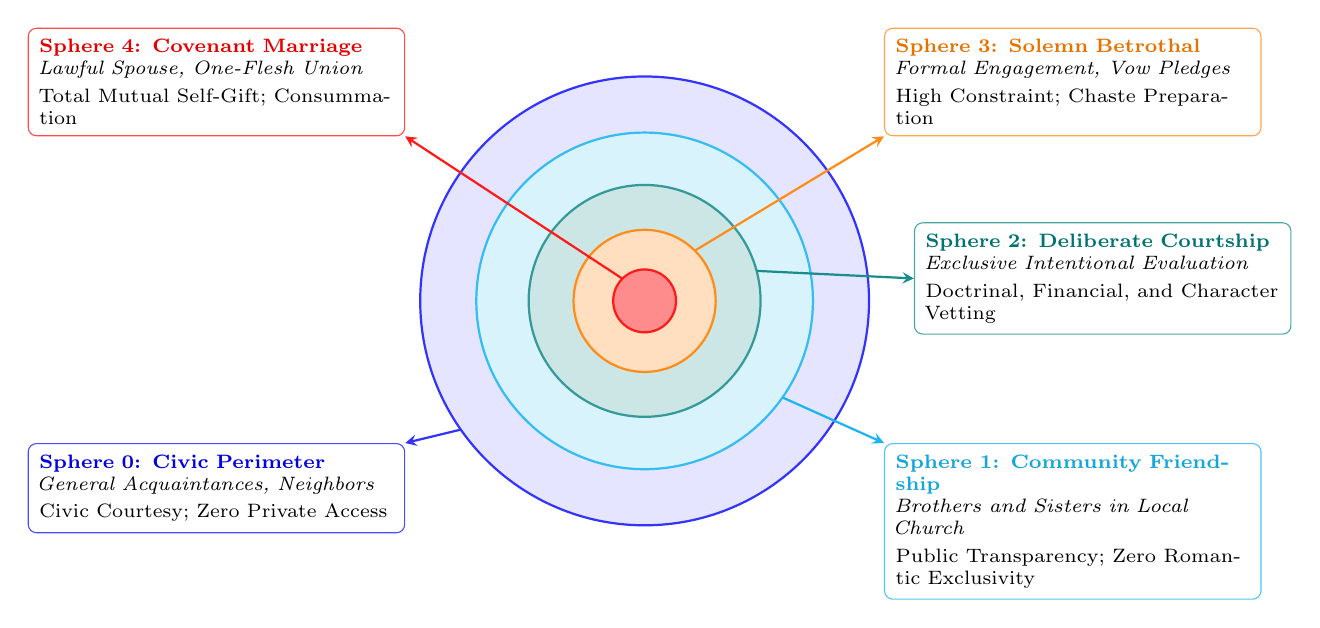
\begin{tikzpicture}[scale=0.95, >=stealth]
  % Concentric rings
  \fill[blue!10] (0,0) circle (3.0cm);
  \fill[cyan!15] (0,0) circle (2.25cm);
  \fill[teal!20] (0,0) circle (1.55cm);
  \fill[orange!25] (0,0) circle (0.95cm);
  \fill[red!45] (0,0) circle (0.42cm);

  \draw[thick, blue!80] (0,0) circle (3.0cm);
  \draw[thick, cyan!80] (0,0) circle (2.25cm);
  \draw[thick, teal!80] (0,0) circle (1.55cm);
  \draw[thick, orange!90] (0,0) circle (0.95cm);
  \draw[thick, red!90] (0,0) circle (0.42cm);

  % Sphere 4 (Marriage - Core)
  \draw[thick, red!90, ->] (135:0.42cm) to (-3.2, 2.2);
  \node[anchor=south east, font=\scriptsize, fill=white, draw=red!70, rounded corners=3pt, inner sep=4pt, text width=4.5cm, align=left] at (-3.2, 2.2) {
    \textbf{\textcolor{red!90!black}{Sphere 4: Covenant Marriage}}\\
    \textit{Lawful Spouse, One-Flesh Union}\\[2pt]
    Total Mutual Self-Gift; Consummation
  };

  % Sphere 3 (Betrothal)
  \draw[thick, orange!90, ->] (45:0.95cm) to (3.2, 2.2);
  \node[anchor=south west, font=\scriptsize, fill=white, draw=orange!70, rounded corners=3pt, inner sep=4pt, text width=4.5cm, align=left] at (3.2, 2.2) {
    \textbf{\textcolor{orange!90!black}{Sphere 3: Solemn Betrothal}}\\
    \textit{Formal Engagement, Vow Pledges}\\[2pt]
    High Constraint; Chaste Preparation
  };

  % Sphere 2 (Courtship)
  \draw[thick, teal!90, ->] (15:1.55cm) to (3.6, 0.3);
  \node[anchor=west, font=\scriptsize, fill=white, draw=teal!70, rounded corners=3pt, inner sep=4pt, text width=4.5cm, align=left] at (3.6, 0.3) {
    \textbf{\textcolor{teal!90!black}{Sphere 2: Deliberate Courtship}}\\
    \textit{Exclusive Intentional Evaluation}\\[2pt]
    Doctrinal, Financial, and Character Vetting
  };

  % Sphere 1 (Friendship)
  \draw[thick, cyan!90, ->] (325:2.25cm) to (3.2, -1.9);
  \node[anchor=north west, font=\scriptsize, fill=white, draw=cyan!70, rounded corners=3pt, inner sep=4pt, text width=4.5cm, align=left] at (3.2, -1.9) {
    \textbf{\textcolor{cyan!90!black}{Sphere 1: Community Friendship}}\\
    \textit{Brothers and Sisters in Local Church}\\[2pt]
    Public Transparency; Zero Romantic Exclusivity
  };

  % Sphere 0 (Perimeter)
  \draw[thick, blue!80, ->] (215:3.0cm) to (-3.2, -1.9);
  \node[anchor=north east, font=\scriptsize, fill=white, draw=blue!70, rounded corners=3pt, inner sep=4pt, text width=4.5cm, align=left] at (-3.2, -1.9) {
    \textbf{\textcolor{blue!90!black}{Sphere 0: Civic Perimeter}}\\
    \textit{General Acquaintances, Neighbors}\\[2pt]
    Civic Courtesy; Zero Private Access
  };
\end{tikzpicture}
\caption{\textbf{The Five Concentric Spheres of Christian Relational Escalation.} Radial boundaries establish strict operational access and information governance from the civic perimeter (Sphere 0) to indissoluble covenant marriage (Sphere 4).}
\label{fig:concentric}
\end{figure*}

\subsection{The Concentric Boundary Topology}
Relational access is governed by five concentric boundary spheres (Figure~\ref{fig:concentric}):
\begin{enumerate}
    \item \textbf{Sphere 0 (Civic Perimeter)}: General acquaintances, civic neighbors, public contacts. Universal courtesy, zero private access.
    \item \textbf{Sphere 1 (Community Friendship)}: Brothers and sisters in the local church. Mutual fellowship, public transparency, collective service, zero romantic exclusivity.
    \item \textbf{Sphere 2 (Deliberate Courtship)}: Exclusive, intentional evaluation of marriageability. Deep theological, moral, financial, and emotional vetting under pastoral and family oversight. Emotional vulnerability calibrated strictly to commitment.
    \item \textbf{Sphere 3 (Solemn Betrothal)}: Public, formal engagement (\textit{sponsalia de futuro}). Finalized legal and logistical preparation, marital counseling, explicit mutual vow pledge without sexual consummation.
    \item \textbf{Sphere 4 (Covenant Marriage)}: Public exchange of vows (\textit{per verba de praesenti}), ecclesiastical blessing, and physical consummation. Complete mutual self-gift (\textit{communio personarum}), permanent structural and emotional union under God.
\end{enumerate}

\begin{eli5box}
\textbf{EXPLAIN LIKE I'M FIVE: The Castle Walls}\\
Think of your heart and your life like a castle with five walls. Outside the outermost wall is the public road. Anyone can walk on the road, and you wave politely to them. That is being a good neighbor. 

Inside the first wall is the castle courtyard. That is where your church friends gather to sing, talk, and help each other. Inside the second wall is the castle library. You only invite one special person in there when both of you are asking: ``Could we build a life together for God?'' In that room, you talk about serious things, like faith, family, money, and fears. 

Inside the third wall is the council chamber. That is engagement, where you make a public promise to marry. Finally, at the very center of the castle is the private hearth room. Only your husband or wife can enter that room on your wedding day. 

The biggest rule of the castle is: no one enters the hearth room until the holy wedding vows are spoken before God and the church. If you open that door early, you lose your castle's protection, and your judgment gets clouded by feelings that deceive you. Keeping the door locked until marriage protects your heart and ensures you marry someone who truly honors God.
\end{eli5box}

\section{Formal Analytical and Game-Theoretic Modeling}

\subsection{Contractual Exchange versus Covenantal Alignment}
Game theory models human interactions through payoffs and information structures. Modern dating operates as a finite, repeated prisoner's dilemma characterized by contractual exchange. In a contract, an agent maximizes discounted selfish utility:
\begin{equation}
U_{\text{contract}} = \sum_{t=0}^{T} \delta^t \Big( \pi_i(a_{i,t}, a_{j,t}) - c_i(a_{i,t}) \Big)
\end{equation}
where agents cooperate solely while the perceived benefit exceeds alternative market opportunities. If partner $j$ experiences illness, financial distress, or loss of physical attractiveness, partner $i$ possesses an incentive to defect.

In contrast, Christian covenant marriage transforms the payoff topology into an infinite-horizon game with irreversible commitment:
\begin{equation}
U_{\text{covenant}} = \mathbb{E} \left[ \sum_{t=0}^{\infty} \beta^t \Big( W(s_t) + \lambda \cdot M_j(s_t) \Big) \right]
\end{equation}
where $\lambda \ge 1$ represents sacrificial agape love (valuing the spouse's eternal and earthly good equally or greater than one's own), and $W(s_t)$ represents obedience to divine covenant.

\subsection{Payoff Matrix of Courtship Integrity}
Consider the normal-form stage game between Suitor ($A$) and Pursued ($B$) during courtship evaluation. Each agent chooses between \textbf{Sober Fidelity} ($C$, honest character disclosure, respecting physical boundaries, honoring accountability) and \textbf{Deceptive Exploitation} ($D$, masking character flaws, feigning piety, seeking sexual gratification without covenant):

\begin{table}[H]
\centering
\caption{Payoff Matrix of Courtship Strategies}
\label{tab:payoff}
\resizebox{\columnwidth}{!}{%
\begin{tabular}{lcc}
\toprule
Suitor ($A$) / Pursued ($B$) & Fidelity ($C$) & Exploitation ($D$) \\
\midrule
Fidelity ($C$) & $(+10, +10)$ & $(-15, +12)$ \\
Exploitation ($D$) & $(+12, -15)$ & $(-8, -8)$ \\
\bottomrule
\end{tabular}%
}
\end{table}

In an unconstrained, secular dating market where physical intimacy occurs freely, the temptation payoff exceeds mutual cooperation ($12 > 10$), creating a dominant strategy to defect, exploiting vulnerability and generating high rates of heartbreak, betrayal, and divorce. 

The Christian courtship framework alters the payoff structure by introducing ecclesiastical oversight, community monitoring, and strict physical boundaries. These measures impose severe social, spiritual, and reputational penalties ($K_{\text{church}} = 25$) upon defection, converting the game into a coordination assurance game where mutual fidelity ($C, C$) is the unique Pareto-dominant subgame-perfect equilibrium:
\begin{equation}
\text{Payoff}(D, C) = 12 - 25 = -13 < +10
\end{equation}

\subsection{The Character Verification Function and State Transition Logic}
Let $V_c(t)$ represent the verified character score of a candidate at time $t$, derived from longitudinal observations across $M$ distinct moral domains (truthfulness, financial stewardship, impulse control, theological orthodoxy, filial honor, and mercy under stress):
\begin{equation}
V_c(t) = \sum_{k=1}^{M} w_k \cdot \int_{0}^{t} \mu_k(\tau) e^{-\gamma (t - \tau)} \, d\tau
\end{equation}
where $w_k$ denotes the domain weight ($\sum w_k = 1$), $\mu_k(\tau) \in [0, 1]$ represents verified behavioral performance, and $\gamma$ is a decay parameter penalizing inconsistent recent behavior.

\begin{figure}[H]
\centering
\resizebox{\columnwidth}{!}{
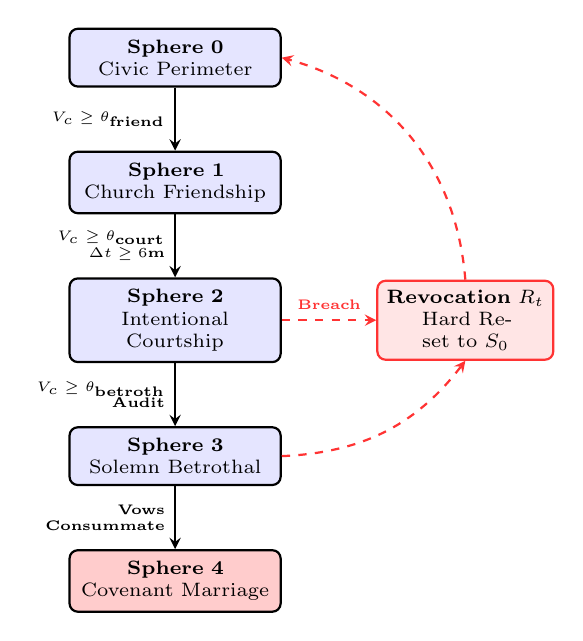
\begin{tikzpicture}[auto, >=stealth,
  snode/.style={rectangle, rounded corners=3pt, draw=black, thick, fill=blue!10, text width=2.4cm, text centered, font=\scriptsize, inner sep=4pt}]

  \node[snode] (s0) {\textbf{Sphere 0}\\Civic Perimeter};
  \node[snode, below=0.8cm of s0] (s1) {\textbf{Sphere 1}\\Church Friendship};
  \node[snode, below=0.8cm of s1] (s2) {\textbf{Sphere 2}\\Intentional Courtship};
  \node[snode, below=0.8cm of s2] (s3) {\textbf{Sphere 3}\\Solemn Betrothal};
  \node[snode, below=0.8cm of s3, fill=red!20] (s4) {\textbf{Sphere 4}\\Covenant Marriage};

  \draw[->, thick] (s0) to node[left, font=\tiny\bfseries] {$V_c \ge \theta_{\text{friend}}$} (s1);
  \draw[->, thick] (s1) to node[left, font=\tiny\bfseries, align=right] {$V_c \ge \theta_{\text{court}}$\\$\Delta t \ge 6\text{m}$} (s2);
  \draw[->, thick] (s2) to node[left, font=\tiny\bfseries, align=right] {$V_c \ge \theta_{\text{betroth}}$\\Audit} (s3);
  \draw[->, thick] (s3) to node[left, font=\tiny\bfseries, align=right] {Vows\\Consummate} (s4);

  \node[rectangle, rounded corners=3pt, draw=red!80, thick, fill=red!10, text width=2.0cm, text centered, font=\scriptsize, right=1.2cm of s2] (revoc) {\textbf{Revocation $R_t$}\\Hard Reset to $S_0$};

  \draw[->, thick, red!80, dashed] (s2.east) to node[above, font=\tiny\bfseries] {Breach} (revoc.west);
  \draw[->, thick, red!80, dashed] (s3.east) to [bend right=25] (revoc.south);
  \draw[->, thick, red!80, dashed] (revoc.north) to [bend right=35] (s0.east);
\end{tikzpicture}
}
\caption{\textbf{Courtship State Machine.} Progression occurs exclusively through verified character thresholds. Deceit or boundary violations trigger immediate revocation.}
\label{fig:statemachine}
\end{figure}

State transitions are governed by strict threshold triggers (Figure~\ref{fig:statemachine}):
\begin{enumerate}
    \item \textbf{Transition $S_0 \to S_1$ (Friendship)}: Requires baseline civic peace and verified reputation: $V_c(t) \ge \theta_{\text{friend}}$.
    \item \textbf{Transition $S_1 \to S_2$ (Courtship)}: Requires longitudinal observation within church community ($\Delta t \ge 6 \text{ months}$), explicit mutual declaration of marital intent, pastoral blessing, and parental concurrence: $V_c(t) \ge \theta_{\text{court}}$.
    \item \textbf{Transition $S_2 \to S_3$ (Betrothal)}: Requires comprehensive financial audit, premarital counseling clearance, verified physical purity, and unanimous elder affirmation: $V_c(t) \ge \theta_{\text{betroth}}$.
    \item \textbf{Transition $S_3 \to S_4$ (Marriage)}: Public exchange of vows (\textit{per verba de praesenti}), ecclesiastical solemnization, legal recording, and sexual consummation.
\end{enumerate}

\subsection{Quarantine and Revocation Mechanics}
If at any point during $S_1, S_2,$ or $S_3$ an agent commits deceit, boundary violation, or moral compromise:
\begin{itemize}
    \item \textbf{Quarantine Trigger ($Q_p$)}: Triggered when $V_c(t) < \theta_{\text{quarantine}}$ or upon an unverified red flag. All relational escalation halts instantly. Interaction drops to public settings only under pastoral supervision for a probationary window ($\Delta t_{\text{prob}} = 90 \text{ days}$).
    \item \textbf{Instant Revocation Trigger ($R_t$)}: Triggered upon unrepentant lying, physical boundary transgression, clandestine manipulation, or discovered infidelity. The state machine executes an immediate hard reset: state reverts to $S_0$, and verified character score drops to zero. All courtship privileges terminate unconditionally.
\end{itemize}

\begin{eli5box}
\textbf{EXPLAIN LIKE I'M FIVE: The Ship Captain's Test}\\
Imagine you want to hire a captain to sail a very precious ship across the ocean. You do not just hand him the keys because he wears a handsome uniform and tells funny jokes. A bad captain can sink your ship.

First, you watch him work on the docks for months. Does he show up on time? Does he tell the truth when he makes a mistake? Does he keep his temper when the wind blows hard? That is measuring his character score. 

Second, you have rules. If he touches the cargo without permission, or if you catch him lying about his experience, you stop everything. You put him in quarantine or tell him to leave the shipyard immediately. 

In courtship, your heart, your future children, and your walk with God are that precious ship. You only advance toward marriage when a person proves across months of real life that they are honest, faithful, and obedient to God. And you never compromise on the safety rules.
\end{eli5box}

\section{Operational Protocols and Real-World Empirical Scenarios}

\subsection{The Three-Phase Courtship Protocol}
\begin{enumerate}
    \item \textbf{Phase 1: Community Friendship and Public Observation ($S_1$)}: Candidate operates within the natural life of the local church and Christian community. Observation focuses on unvarnished behavior: how the candidate treats parents, handles financial pressure, exercises speech under frustration, and serves without public praise. No romantic exclusivity, no late-night private communications, no physical touch beyond civic greeting.
    \item \textbf{Phase 2: Intentional Deliberate Courtship ($S_2$)}: Explicit directional conversation initiating courtship: ``I admire your godly character and desire to evaluate marriage with you under church and family accountability.'' Structured private dialogue centered on doctrinal convictions, debt and spending habits, child-rearing philosophy, and past wounds. Physical boundary protocol: Chaste public interaction only. No secluded domestic isolation. Group and family settings remain the primary locus of activity.
    \item \textbf{Phase 3: Formal Betrothal and Premarital Preparation ($S_3$)}: Public proposal and exchange of betrothal pledges. Formal premarital counseling covering theological roles, conflict resolution, sexual ethics within marriage, and financial integration. Final preparation of household, wedding liturgy, and ecclesiastical blessing.
\end{enumerate}

\subsection{Handling Relational Adversity: Deception, Infidelity, and Repentance}
Spouses and suitors are fallen humans. When deceit or betrayal emerges:
\begin{itemize}
    \item \textbf{Pre-Marriage Discovery}: If lying, sexual infidelity, or hidden debt surfaces during $S_1, S_2,$ or $S_3$, the innocent party must execute the Revocation Trigger ($R_t$). Forgiveness must be granted spiritually (clearing malice and bitterness, Matthew 18:21-22), yet trust is not restored. Courtship terminates. Trust is an earned stewardship; it is never an unconditional entitlement.
    \item \textbf{Post-Marriage Breach (Adultery / Abandonment)}: Within covenant marriage ($S_4$), adultery constitutes a grave violation of the marriage bed (Hebrews 13:4). The wronged spouse may seek reconciliation through deep pastoral intervention and biblical repentance. If the offending spouse remains unrepentant or if an unbelieving spouse departs (1 Corinthians 7:15, Westminster Confession 24.6), biblical grounds for divorce apply, releasing the innocent party.
\end{itemize}

\begin{eli5box}
\textbf{EXPLAIN LIKE I'M FIVE: Forgiving the Broken Watch}\\
What happens if someone you are dating tells you a lie or cheats on you? 

Jesus teaches us to forgive people in our hearts so that bitterness does not poison our soul. You release the anger and pray for them. Forgiving someone does not require marrying them. 

If someone drops and breaks a borrowed golden watch, you forgive them for breaking it, but you do not hand them another golden watch the next day. If a suitor lies to you or betrays your trust before marriage, you forgive them, say goodbye, and end the courtship. Before marriage, you have the full freedom and duty to walk away from someone who proves untrustworthy.
\end{eli5box}

\section{Objections, Counter-Arguments, and Edge-Case Failures}

\subsection{The Modernist Objection: The Test Drive Myth}
Modern secular culture argues that couples must cohabit and engage in sexual relations before marriage to determine compatibility. 

\noindent\textbf{Empirical Refutation:} Decades of demographic and sociological data refute this premise. Studies by Scott Stanley, Galena Rhoades, and the National Marriage Project demonstrate that premarital cohabitation increases divorce risk or fails to improve marital stability. Cohabitation generates sliding inertia, where couples marry because of financial friction and shared leases, neglecting verified dedication. Premarital chastity, by contrast, preserves cognitive clarity, ensuring marriage is established on tested character and mutual spiritual commitment.

\subsection{The Legalism Objection: Boundaries and Affection}
Critics claim that objective boundaries, accountability, and elders stifle genuine romance and organic emotional connection.

\noindent\textbf{Theological Refutation:} Biblical wisdom establishes that true love flourishes inside protective boundaries (Proverbs 4:23, 1 Corinthians 13:4-7). Guardrails protect affection from predatory exploitation, emotional manipulation, and premature heartbreak. Freedom exists within holy law, just as a river flows with power and beauty between sturdy banks.

\subsection{The Edge Case of Past Divorce and Relational Grief}
A vital edge case involves believers who experienced a previous divorce, whether through youthful folly or tragic desertion by an unfaithful, unbelieving spouse (1 Corinthians 7:15).

\noindent\textbf{Pastoral Resolution:} Entering courtship after a broken marriage requires profound sobriety. God designed marriage as a lifelong, once-in-a-lifetime union (Genesis 2:24, Malachi 2:16). Divorce represents a grievous rupture of one flesh. An individual seeking second marriage must undergo rigorous pastoral evaluation:
\begin{enumerate}
    \item Complete repentance and grieving over past relational failures.
    \item Full resolution of parental duties toward children from the prior union.
    \item Verification that the previous bond dissolved under biblically legitimate grounds (1 Corinthians 7:15 abandonment or Matthew 19:9 sexual immorality).
    \item Slower, audited courtship progression with intensified elder oversight.
\end{enumerate}

Past failure serves as inverted pedagogy: understanding what destroyed the first union provides the precise vigilance required to protect the future covenant.

\begin{eli5box}
\textbf{EXPLAIN LIKE I'M FIVE: Fire in the Fireplace}\\
Some people say: ``Why have so many rules? Why not just follow your feelings?'' 

Think of a roaring fire. When a fire is inside a strong brick fireplace, it keeps the whole house warm and safe. Children can sit near it, laugh, and read books. But if you take the burning logs out of the fireplace and spread them across the living room carpet, the fire burns the whole house down! 

The rules of courtship: keeping your hands to yourself, involving wise parents and church pastors, and asking hard questions: are the bricks of the fireplace. They keep love warm, beautiful, and safe so that it never burns down your life.
\end{eli5box}

\section{Conclusion, Limitations, and Future Research}

\subsection{Synthesis of Findings}
Christian courtship is an intentional, audited state machine designed to steward human affection toward an unbreakable covenant. By synthesizing the covenantal accountability of the Protestant tradition, the sacramental depth and personalistic norm of the Catholic tradition, and the ascetical watchfulness of the Greek Orthodox tradition, believers can navigate relational formation with holy confidence. Supported by modern commitment theory and family systems differentiation, this framework secures marriages against the pervasive rot of consumerist dating, protecting husbands, wives, and future generations.

\subsection{Limitations and Future Research}
This study models idealized communal and ecclesiastical structures. In highly atomized, urbanized contexts where local church communities lack formal consistories or eldership oversight, operational execution requires creative adaptations, such as Christian parachurch mentoring networks. Future empirical research should quantify the longitudinal marital longevity of cohorts adhering to formal five-stage courtship protocols compared to conventional dating cohorts over twenty-year horizons.

\begin{eli5box}
\textbf{EXPLAIN LIKE I'M FIVE: The Finished House}\\
Building a marriage is the most important construction project of your adult life. If you follow God's blueprints: starting with faithful friendship, moving slowly through careful courtship, testing honesty at every step, and saving the deepest physical affection for marriage: you will build a home that stands strong against every wind and rain.
\end{eli5box}

\begin{thebibliography}{99}
\bibitem{aquinas} Aquinas, Thomas. \textit{Summa Theologiae}, Supplementum, Questions 41 through 68. Translated by the Fathers of the English Dominican Province. New York: Benziger Brothers, 1948.
\bibitem{augustine} Augustine of Hippo. \textit{De Bono Coniugali} (On the Good of Marriage). In \textit{Nicene and Post-Nicene Fathers}, First Series, Vol. 3. Edited by Philip Schaff. Buffalo, NY: Christian Literature Publishing Co., 1887.
\bibitem{baxter} Baxter, Richard. \textit{A Christian Directory: A Sum of Practical Theology and Cases of Conscience}. London: Robert White, 1673.
\bibitem{bowen} Bowen, Murray. \textit{Family Therapy in Clinical Practice}. New York: Jason Aronson, 1978.
\bibitem{calvin} Calvin, John. \textit{Institutes of the Christian Religion}. Edited by John T.~McNeill, translated by Ford Lewis Battles. Philadelphia: Westminster Press, 1960.
\bibitem{chrysostom} Chrysostom, John. \textit{Homilies on the Epistles of Saint Paul to the Ephesians}. In \textit{Nicene and Post-Nicene Fathers}, First Series, Vol. 13. Edited by Philip Schaff. New York: Christian Literature Company, 1889.
\bibitem{johnpaul} John Paul II, Pope (Karol Wojtyla). \textit{Theology of the Body: Human Love in the Divine Plan}. Boston: Pauline Books and Media, 1997.
\bibitem{luther} Luther, Martin. \textit{The Estate of Marriage} (1522). In \textit{Luther's Works}, Vol. 45: The Christian in Society II. Edited by Walther I.~Brandt. Philadelphia: Muhlenberg Press, 1962.
\bibitem{markman} Markman, Howard J., Scott M.~Stanley, and Susan L.~Blumberg. \textit{Fighting for Your Marriage}. San Francisco: Jossey-Bass, 2010.
\bibitem{perkins} Perkins, William. \textit{Christian Oeconomie, or A Short Survey of the Right Manner of Erecting and Ordering a Familie}. London: Felix Kyngston, 1609.
\bibitem{rhoades} Rhoades, Galena K., Scott M.~Stanley, and Howard J.~Markman. ``The Pre-Engagement Cohabitation Effect: A Replication and Extension of Previous Findings.'' \textit{Journal of Family Psychology} 23, no. 1 (2009): pages 107 to 111.
\bibitem{skowron} Skowron, Elizabeth A., and Myrna L.~Friedlander. ``The Differentiation of Self Inventory: Development and Initial Validation.'' \textit{Journal of Counseling Psychology} 45, no. 3 (1998): pages 235 to 246.
\bibitem{stanley1992} Stanley, Scott M., and Howard J.~Markman. ``Assessing Commitment in Personal Relationships.'' \textit{Journal of Marriage and Family} 54, no. 3 (1992): pages 595 to 608.
\bibitem{stanley2006} Stanley, Scott M., Galena K.~Rhoades, and Howard J.~Markman. ``Sliding Versus Deciding: Inertia and the Premarital Cohabitation Effect.'' \textit{Family Relations} 55, no. 4 (2006): pages 499 to 509.
\bibitem{westminster} Westminster Assembly. \textit{The Westminster Confession of Faith}. London: Printed for the Company of Stationers, 1646.
\bibitem{wojtyla} Wojtyla, Karol (Pope John Paul II). \textit{Love and Responsibility}. Translated by H.~T.~Willetts. San Francisco: Ignatius Press, 1981.
\end{thebibliography}

\end{document}
